\chapter{Quantised vortices in droplets}\label{sec:quant-vort}
	\lettrine[lines=4]{\color{activeColor}O}{ne} of the most unambiguous signatures of the quantum mechanical nature of a substance---and indeed superfluidity---is the appearance of quantised vortices. The work in this part of the thesis is mostly inspired and motivated by experiments performed by Gomez, Loginov and Vilesov\citep{Gomez:2012,Gom14}. 
	
	Normal fluids rotate rigidly when their containers are spinning at low angular velocities, with an angular velocity $v_\perp$ proportional to the distance $r$ from the axis of rotation $v_\perp\propto r$. This behaviour changes completely when the normal fluid is replaced by a superfluid like liquid helium below $T_\lambda$; below a critical angular velocity, the fluid remains at rest. When the angular velocity of the container is increased above this critical velocity, one or more quantised vortices are nucleated. In contrast to the angular velocity a normal fluid, the angular velocity $v_s$ directly outside the vortex core is inverse proportional to the distance from the vortex core $v_s\propto 1/r$. These vortices can be described by an effective wave function and a quantised circulation $\Gamma$ in the velocity field
	\begin{align}
		\Gamma=s\frac{h}{m}	
	\end{align}
	where $s$ is the angular momentum quantum number, $h$ is Planck’s constant and $m$ is the mass of the $^4$He atom (see \eq{eq:circulation} for a derivation and\rfs{Don91,Pit03}). An important aspect in the study of vorticity in finite systems is the energy and momentum transfer between vortices and surface excitations, because they determine nucleation dynamics, shape and he stability of vortices. But the study of quantum vortices is no longer confined to superfluids like liquid helium. Recently\citep{Pit03,Fetter2009} it has been extended to BECs confined in magnetic traps. Contrary to confined BECs, superfluid helium droplets are self-contained systems that do not require an external trap. Moreover, they provide an opportunity to study the regime of  strongly interacting quantum systems. The size of vortex cores, about 0.2~nm\citep{Don91} in superfluid helium-4, is small compared to size of the droplets (typically a diameter of $\sim$4.4--10.9~nm), suggesting a rich variety of three-dimensional phenomena. Quantum vortices in superfluid droplets are therefore a very active field of interest\citep{Clo98,Lehmann2003,Bar06,Sti06}. 
	
	Recently, Gomez \emph{et al}. performed experiments\citep{Gomez:2012} where vortices inside superfluid $^4$He nanodroplets, produced by the expansion of liquid helium, were doped with Ag atoms which then clustered along the vortex lines in the droplets. The helium droplets needed by these kind of experiments need to be larger than used before for single atom spectroscopy and dynamics studies because they need to be big enough to be able to host an array of vortices, doped with many Ag clusters.
	
	A schematic of the experimental principle is shown in \fig{fig:vortex-machine}. Helium droplets are produced by expansion of He, at 20~bar and a temperature $T_0$=5.4--7~K, into a vacuum through a nozzle. The droplets cool down rapidly by evaporation and reach a temperature of 0.37~K\citep{Hartmann1995}. This temperature is well below the superfluid transition temperature $T_\lambda$=2.17~K\citep{Don91,Pit03}. Further along the apparatus, the droplets capture about 10$^3$–10$^6$~Ag atoms in an oven\citep{Log11d}. The droplets are then collided against a thin carbon film substrate at room temperature\citep{Log11d}. When the droplets hit the carbon film they evaporate while leaving behind on the surface the Ag filaments, which are subsequently imaged via a transmission electron microscope (TEM).
	
	The ubiquity of elongated filament-shaped deposits (see \fig{fig:silver-filament}) shows that vortices are present in droplets larger than about 300~nm and that their lifetime exceeds a few milliseconds.
	
	\begin{figure}[t]
		\begin{center}
			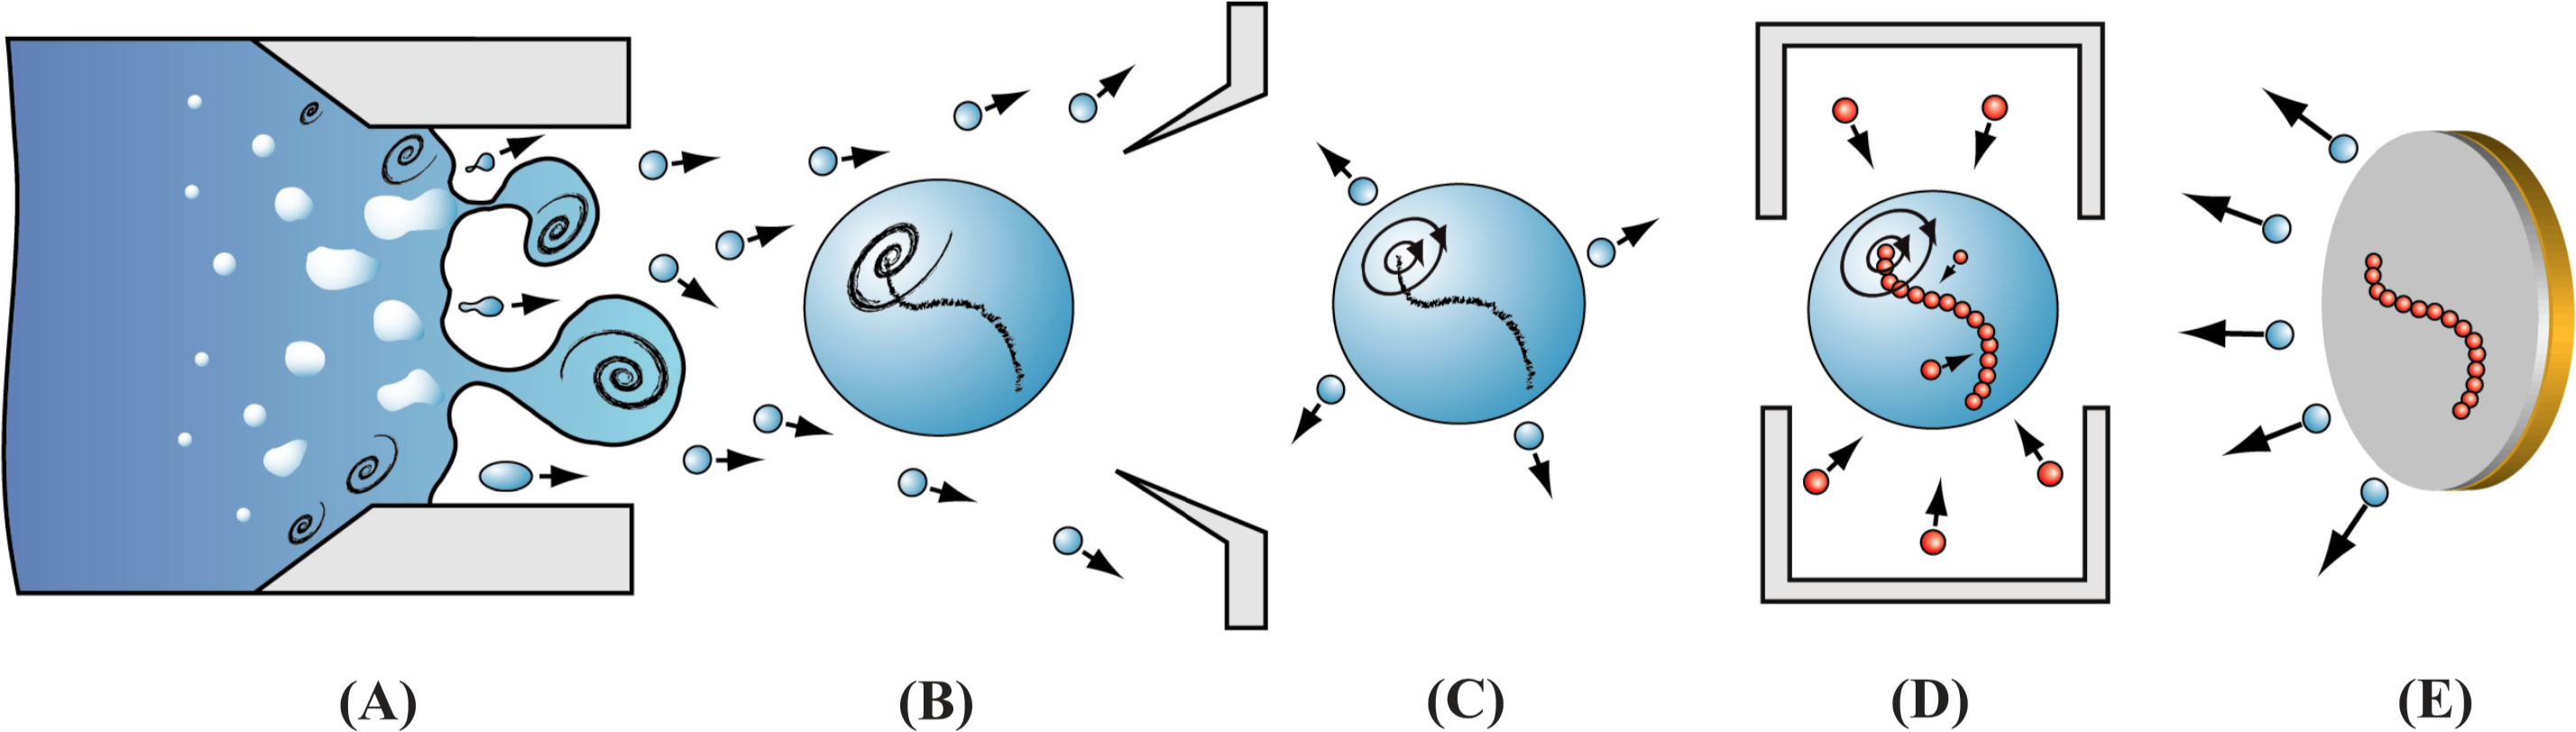
\includegraphics[width=\textwidth]{vortex-machine}
			\caption{Schematic of the experiment. (a) He fluid expands in vacuum and (b) breaks up into rotating droplets. (c) A quantum vortex is formed as a consequence of fast evaporative cooling of the droplet to below $T_\lambda$. (d) The droplet is doped with Ag atoms, which are attracted to the vortex core. (e) The droplet then collides with the carbon surface leaving behind the Ag trace, whereas the He evaporates. (Illustration courtesy of Gomez \emph{et al}. 2012, see\rf{Gomez:2012})}
			\label{fig:vortex-machine}
		\end{center}
	\end{figure}	
	
	Two years later Gomez \emph{et al}. reported\citep{Gom14} on the formation of quantum vortex lattices inside droplets. They used single-shot femtosecond X-ray coherent diffractive imaging to investigate the rotation of single, isolated superfluid helium-4 droplets containing about 10$^8$--10$^{11}$ atoms. The formation of quantum vortex lattices inside the droplets was confirmed by observing the characteristic Bragg patterns from xenon clusters trapped in the vortex cores (see \fig{fig:vortex-array}).

	\begin{figure}[t]
		\begin{center}
			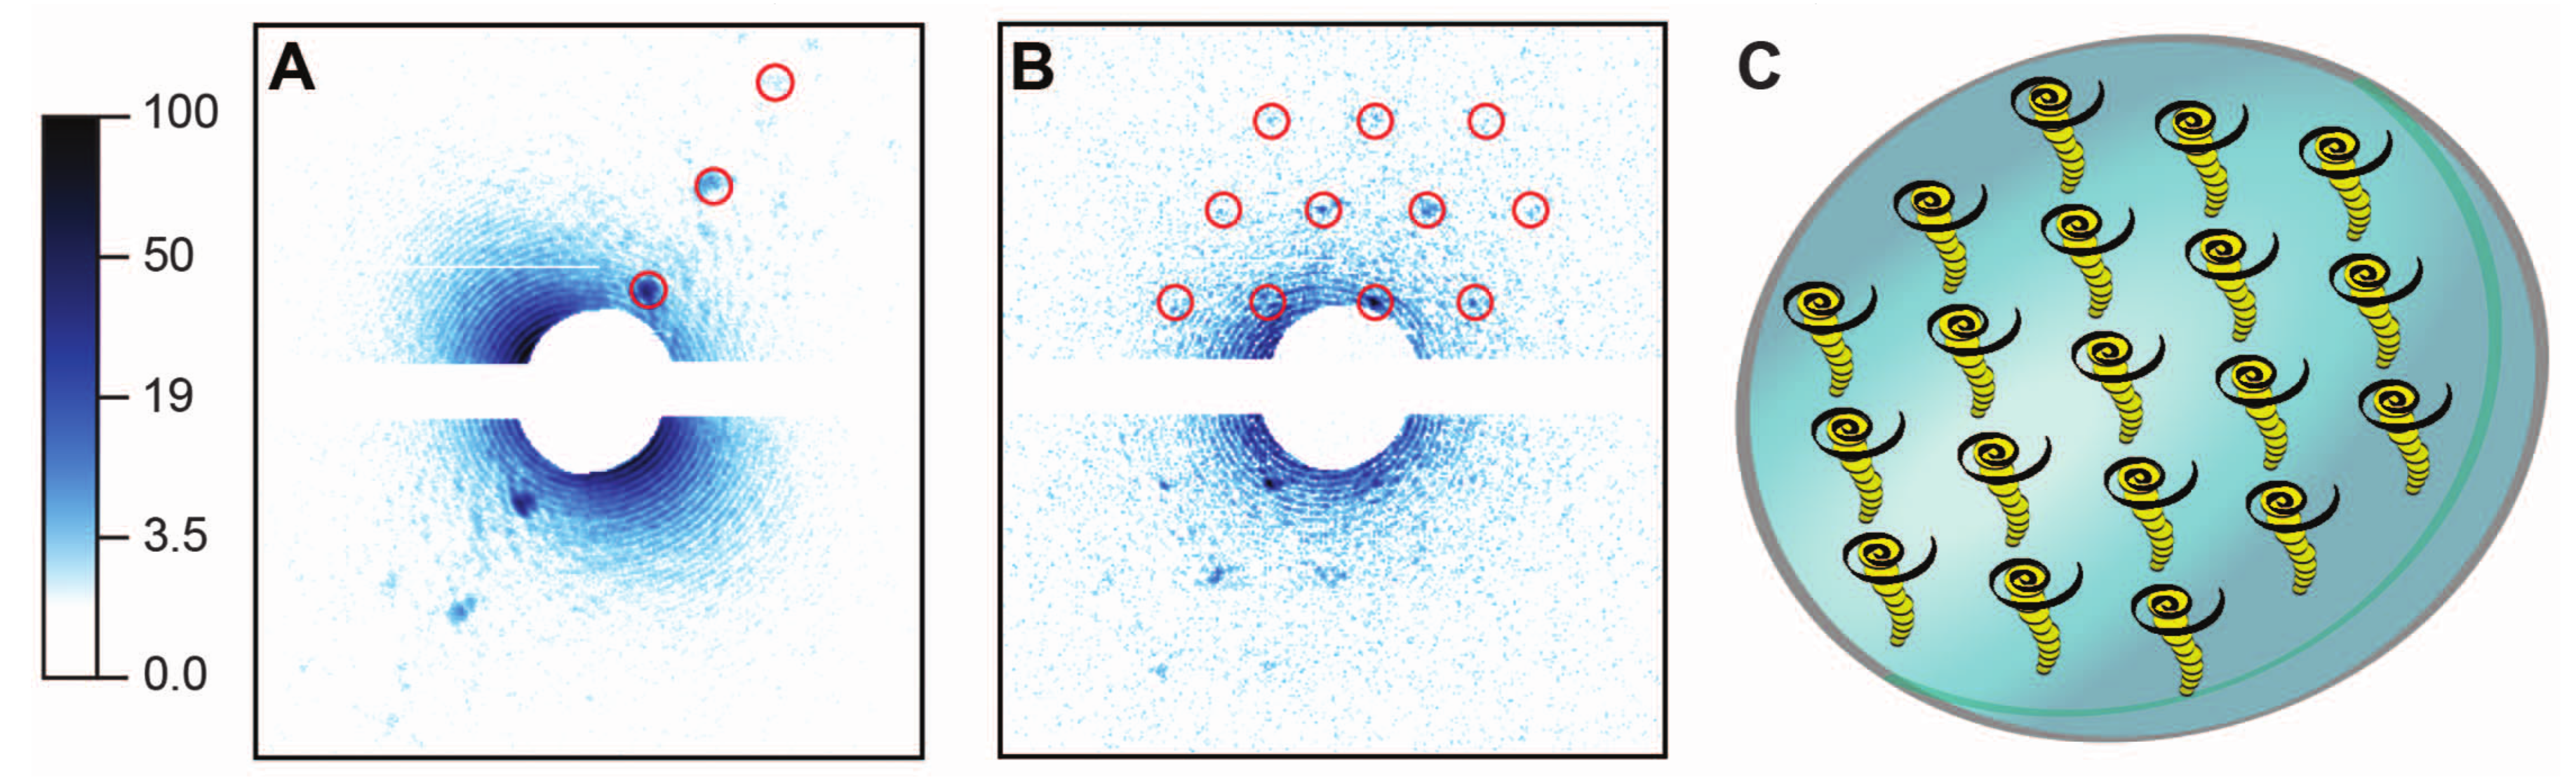
\includegraphics[width=\textwidth]{vortex-array}
			\caption{He droplets doped with Xe atoms. (A and B) X-ray diffraction images of doped droplets, displayed in a logarithmic intensity scale. (C) Droplet and embedded Xe clusters. Images in (A) and (B) correspond to tilted and parallel alignments of the vortex axes with respect to the incident x-ray beam, respectively. (Illustration courtesy of Gomez \emph{et al}. 2014, see\rf{Gom14})}
			\label{fig:vortex-array}
		\end{center}
	\end{figure}
\clearpage{\pagestyle{empty}\cleardoublepage}